% Generated by Sphinx.
\def\sphinxdocclass{report}
\documentclass[letterpaper,10pt,english]{sphinxmanual}
\usepackage[utf8]{inputenc}
\DeclareUnicodeCharacter{00A0}{\nobreakspace}
\usepackage[T1]{fontenc}
\usepackage{babel}
\usepackage{times}
\usepackage[Bjarne]{fncychap}
\usepackage{longtable}
\usepackage{sphinx}
\usepackage{multirow}
\usepackage{bera}

\title{django-textvariation Documentation}
\date{July 08, 2011}
\release{0.1}
\author{Corey Oordt}
\newcommand{\sphinxlogo}{}
\renewcommand{\releasename}{Release}
\makeindex

\makeatletter
\def\PYG@reset{\let\PYG@it=\relax \let\PYG@bf=\relax%
    \let\PYG@ul=\relax \let\PYG@tc=\relax%
    \let\PYG@bc=\relax \let\PYG@ff=\relax}
\def\PYG@tok#1{\csname PYG@tok@#1\endcsname}
\def\PYG@toks#1+{\ifx\relax#1\empty\else%
    \PYG@tok{#1}\expandafter\PYG@toks\fi}
\def\PYG@do#1{\PYG@bc{\PYG@tc{\PYG@ul{%
    \PYG@it{\PYG@bf{\PYG@ff{#1}}}}}}}
\def\PYG#1#2{\PYG@reset\PYG@toks#1+\relax+\PYG@do{#2}}

\def\PYG@tok@gd{\def\PYG@tc##1{\textcolor[rgb]{0.63,0.00,0.00}{##1}}}
\def\PYG@tok@gu{\let\PYG@bf=\textbf\def\PYG@tc##1{\textcolor[rgb]{0.50,0.00,0.50}{##1}}}
\def\PYG@tok@gt{\def\PYG@tc##1{\textcolor[rgb]{0.00,0.25,0.82}{##1}}}
\def\PYG@tok@gs{\let\PYG@bf=\textbf}
\def\PYG@tok@gr{\def\PYG@tc##1{\textcolor[rgb]{1.00,0.00,0.00}{##1}}}
\def\PYG@tok@cm{\let\PYG@it=\textit\def\PYG@tc##1{\textcolor[rgb]{0.25,0.50,0.56}{##1}}}
\def\PYG@tok@vg{\def\PYG@tc##1{\textcolor[rgb]{0.73,0.38,0.84}{##1}}}
\def\PYG@tok@m{\def\PYG@tc##1{\textcolor[rgb]{0.13,0.50,0.31}{##1}}}
\def\PYG@tok@mh{\def\PYG@tc##1{\textcolor[rgb]{0.13,0.50,0.31}{##1}}}
\def\PYG@tok@cs{\def\PYG@tc##1{\textcolor[rgb]{0.25,0.50,0.56}{##1}}\def\PYG@bc##1{\colorbox[rgb]{1.00,0.94,0.94}{##1}}}
\def\PYG@tok@ge{\let\PYG@it=\textit}
\def\PYG@tok@vc{\def\PYG@tc##1{\textcolor[rgb]{0.73,0.38,0.84}{##1}}}
\def\PYG@tok@il{\def\PYG@tc##1{\textcolor[rgb]{0.13,0.50,0.31}{##1}}}
\def\PYG@tok@go{\def\PYG@tc##1{\textcolor[rgb]{0.19,0.19,0.19}{##1}}}
\def\PYG@tok@cp{\def\PYG@tc##1{\textcolor[rgb]{0.00,0.44,0.13}{##1}}}
\def\PYG@tok@gi{\def\PYG@tc##1{\textcolor[rgb]{0.00,0.63,0.00}{##1}}}
\def\PYG@tok@gh{\let\PYG@bf=\textbf\def\PYG@tc##1{\textcolor[rgb]{0.00,0.00,0.50}{##1}}}
\def\PYG@tok@ni{\let\PYG@bf=\textbf\def\PYG@tc##1{\textcolor[rgb]{0.84,0.33,0.22}{##1}}}
\def\PYG@tok@nl{\let\PYG@bf=\textbf\def\PYG@tc##1{\textcolor[rgb]{0.00,0.13,0.44}{##1}}}
\def\PYG@tok@nn{\let\PYG@bf=\textbf\def\PYG@tc##1{\textcolor[rgb]{0.05,0.52,0.71}{##1}}}
\def\PYG@tok@no{\def\PYG@tc##1{\textcolor[rgb]{0.38,0.68,0.84}{##1}}}
\def\PYG@tok@na{\def\PYG@tc##1{\textcolor[rgb]{0.25,0.44,0.63}{##1}}}
\def\PYG@tok@nb{\def\PYG@tc##1{\textcolor[rgb]{0.00,0.44,0.13}{##1}}}
\def\PYG@tok@nc{\let\PYG@bf=\textbf\def\PYG@tc##1{\textcolor[rgb]{0.05,0.52,0.71}{##1}}}
\def\PYG@tok@nd{\let\PYG@bf=\textbf\def\PYG@tc##1{\textcolor[rgb]{0.33,0.33,0.33}{##1}}}
\def\PYG@tok@ne{\def\PYG@tc##1{\textcolor[rgb]{0.00,0.44,0.13}{##1}}}
\def\PYG@tok@nf{\def\PYG@tc##1{\textcolor[rgb]{0.02,0.16,0.49}{##1}}}
\def\PYG@tok@si{\let\PYG@it=\textit\def\PYG@tc##1{\textcolor[rgb]{0.44,0.63,0.82}{##1}}}
\def\PYG@tok@s2{\def\PYG@tc##1{\textcolor[rgb]{0.25,0.44,0.63}{##1}}}
\def\PYG@tok@vi{\def\PYG@tc##1{\textcolor[rgb]{0.73,0.38,0.84}{##1}}}
\def\PYG@tok@nt{\let\PYG@bf=\textbf\def\PYG@tc##1{\textcolor[rgb]{0.02,0.16,0.45}{##1}}}
\def\PYG@tok@nv{\def\PYG@tc##1{\textcolor[rgb]{0.73,0.38,0.84}{##1}}}
\def\PYG@tok@s1{\def\PYG@tc##1{\textcolor[rgb]{0.25,0.44,0.63}{##1}}}
\def\PYG@tok@gp{\let\PYG@bf=\textbf\def\PYG@tc##1{\textcolor[rgb]{0.78,0.36,0.04}{##1}}}
\def\PYG@tok@sh{\def\PYG@tc##1{\textcolor[rgb]{0.25,0.44,0.63}{##1}}}
\def\PYG@tok@ow{\let\PYG@bf=\textbf\def\PYG@tc##1{\textcolor[rgb]{0.00,0.44,0.13}{##1}}}
\def\PYG@tok@sx{\def\PYG@tc##1{\textcolor[rgb]{0.78,0.36,0.04}{##1}}}
\def\PYG@tok@bp{\def\PYG@tc##1{\textcolor[rgb]{0.00,0.44,0.13}{##1}}}
\def\PYG@tok@c1{\let\PYG@it=\textit\def\PYG@tc##1{\textcolor[rgb]{0.25,0.50,0.56}{##1}}}
\def\PYG@tok@kc{\let\PYG@bf=\textbf\def\PYG@tc##1{\textcolor[rgb]{0.00,0.44,0.13}{##1}}}
\def\PYG@tok@c{\let\PYG@it=\textit\def\PYG@tc##1{\textcolor[rgb]{0.25,0.50,0.56}{##1}}}
\def\PYG@tok@mf{\def\PYG@tc##1{\textcolor[rgb]{0.13,0.50,0.31}{##1}}}
\def\PYG@tok@err{\def\PYG@bc##1{\fcolorbox[rgb]{1.00,0.00,0.00}{1,1,1}{##1}}}
\def\PYG@tok@kd{\let\PYG@bf=\textbf\def\PYG@tc##1{\textcolor[rgb]{0.00,0.44,0.13}{##1}}}
\def\PYG@tok@ss{\def\PYG@tc##1{\textcolor[rgb]{0.32,0.47,0.09}{##1}}}
\def\PYG@tok@sr{\def\PYG@tc##1{\textcolor[rgb]{0.14,0.33,0.53}{##1}}}
\def\PYG@tok@mo{\def\PYG@tc##1{\textcolor[rgb]{0.13,0.50,0.31}{##1}}}
\def\PYG@tok@mi{\def\PYG@tc##1{\textcolor[rgb]{0.13,0.50,0.31}{##1}}}
\def\PYG@tok@kn{\let\PYG@bf=\textbf\def\PYG@tc##1{\textcolor[rgb]{0.00,0.44,0.13}{##1}}}
\def\PYG@tok@o{\def\PYG@tc##1{\textcolor[rgb]{0.40,0.40,0.40}{##1}}}
\def\PYG@tok@kr{\let\PYG@bf=\textbf\def\PYG@tc##1{\textcolor[rgb]{0.00,0.44,0.13}{##1}}}
\def\PYG@tok@s{\def\PYG@tc##1{\textcolor[rgb]{0.25,0.44,0.63}{##1}}}
\def\PYG@tok@kp{\def\PYG@tc##1{\textcolor[rgb]{0.00,0.44,0.13}{##1}}}
\def\PYG@tok@w{\def\PYG@tc##1{\textcolor[rgb]{0.73,0.73,0.73}{##1}}}
\def\PYG@tok@kt{\def\PYG@tc##1{\textcolor[rgb]{0.56,0.13,0.00}{##1}}}
\def\PYG@tok@sc{\def\PYG@tc##1{\textcolor[rgb]{0.25,0.44,0.63}{##1}}}
\def\PYG@tok@sb{\def\PYG@tc##1{\textcolor[rgb]{0.25,0.44,0.63}{##1}}}
\def\PYG@tok@k{\let\PYG@bf=\textbf\def\PYG@tc##1{\textcolor[rgb]{0.00,0.44,0.13}{##1}}}
\def\PYG@tok@se{\let\PYG@bf=\textbf\def\PYG@tc##1{\textcolor[rgb]{0.25,0.44,0.63}{##1}}}
\def\PYG@tok@sd{\let\PYG@it=\textit\def\PYG@tc##1{\textcolor[rgb]{0.25,0.44,0.63}{##1}}}

\def\PYGZbs{\char`\\}
\def\PYGZus{\char`\_}
\def\PYGZob{\char`\{}
\def\PYGZcb{\char`\}}
\def\PYGZca{\char`\^}
\def\PYGZsh{\char`\#}
\def\PYGZpc{\char`\%}
\def\PYGZdl{\char`\$}
\def\PYGZti{\char`\~}
% for compatibility with earlier versions
\def\PYGZat{@}
\def\PYGZlb{[}
\def\PYGZrb{]}
\makeatother

\begin{document}

\maketitle
\tableofcontents
\phantomsection\label{index::doc}



\chapter{Goals of Text Variations}
\label{goals:goals-of-text-variations}\label{goals::doc}\label{goals:contents}
Django Text Variations grew out of a need for certain types of content to have multiple versions of text based on specified variation types.

In short, text variations needs to accomplish:
\begin{enumerate}
\item {} 
There can be multiple types of variations (e.g. language, audience, text difficulty)

\item {} 
There could be multiple fields on a model which require text variations.

\item {} 
There could be a maximum number of variations of content equal to the multiplication of the number of each variation type. (e.g. text difficulty levels x audiences x languages)

\item {} 
Variation types are configurable on a per-project (site) implementation.

\item {} 
Any of the variation types, or the variations within that type, could be added to or removed from at any time. (e.g. deciding on going from one language to multiple languages, or going from two language variations to three)

\item {} 
There should be a way to handle addressing the variation in a url.

\item {} 
Not all the variations will be used for each item.

\item {} 
There should be a default variation. If an addressed variation does not exist, it should use the default variation, or a variation algorithmically specified using available variations (graceful fallback).

\item {} 
Invalidation of variations should happen when the default content is changed.

\end{enumerate}


\chapter{Installation}
\label{installation:installation}\label{installation::doc}
Installation is easy using \code{pip} or \code{easy\_install}.

\begin{Verbatim}[commandchars=\\\{\}]
pip install django-textvariation
\end{Verbatim}

or

\begin{Verbatim}[commandchars=\\\{\}]
easy\PYGZus{}install django-textvariation
\end{Verbatim}


\section{Dependencies}
\label{installation:dependencies}
None.


\chapter{Getting Started}
\label{getting_started:getting-started}\label{getting_started::doc}

\section{What are Variations?}
\label{getting_started:what-are-variations}
Textual variations are common in current websites, but are usually only implemented in one dimension: language. Django Text Variations allows you to have text (potentially) vary on multiple dimensions such as language, text difficulty, and audience.

In Django Text Variations, a variation is a specific combination of variants from each dimension.


\subsection{Dimensions}
\label{getting_started:dimensions}
A dimension is one set of ways in which text may vary, such as language. Each dimension has specific ways in which it could vary, such as English and Spanish, called variants.

In further examples, we'll assume that we need text to (potentially) vary on three dimensions.
\begin{itemize}
\item {} 
\textbf{Audiences} with three variants: Adult, Teen, Child

\item {} 
\textbf{Text Difficulty} with three variants: Low, Standard, Advanced

\item {} 
\textbf{Language} with four variants: English, Spanish, Mexican Spanish, French

\end{itemize}


\subsection{Defaults and Graceful Fallback}
\label{getting_started:defaults-and-graceful-fallback}
In many cases, possibly most, you don't need text variations for every possible combination of dimensions. In the case when a specific combination is requested but does does not exist for that object, another variation is delivered. The variation delivered is based on the initial request, the priority of the dimensions, and the available variations.

Django Text Variations is designed to allow for a default, which is the initial text provided, and is assigned to a combination based on the configuration of the dimensions. In the case where no other variations are provided, the default is always delivered.

Within each dimension, there may be a preference in which alternates are resolved. In the case of a language dimension, you may have an object missing a Mexican Spanish variation look first for a Spanish variation, and finally use default English variation. A missing French variation would simply look for an English variation.

\begin{Verbatim}[commandchars=@\[\]]
Mexican Spanish
+-@textgreater[] Spanish
    +-@textgreater[] English

French
+-@textgreater[] English
\end{Verbatim}


\subsection{Configuration of Dimensions and Fallback}
\label{getting_started:configuration-of-dimensions-and-fallback}
Each text variation dimension defines a list of variants. Each variant has a ``code'' or ``slug'', a name, and a fall back variant. One variant should not have a fall back. This is the default variant for the dimension.

\begin{notice}{note}{Note:}
If a dimension contains multiple variants without a fall back variant, strange results may occur.
\end{notice}

Because there are multiple ways to find the next potential variation, if the requested variation is missing, you specify the priority of the dimensions.

So, in our example dimensions, we could define them as:

\begin{tabulary}{\linewidth}{|L|L|L|L|}
\hline
\textbf{
Dimension
} & \textbf{
Name
} & \textbf{
Code
} & \textbf{
Fallback
}\\
\hline
 \multirow{3}{*}{
Audience
} & 
Adult
 & 
ad
 & 
\emph{None}
\\
 & 
Teen
 & 
tn
 & 
Adult
\\
 & 
Child
 & 
cd
 & 
Teen
\\
 \multirow{3}{*}{
Text Difficulty
} & 
Low
 & 
l
 & 
Standard
\\
 & 
Standard
 & 
s
 & 
\emph{None}
\\
 & 
Advanced
 & 
a
 & 
Standard
\\
 \multirow{4}{*}{
Language
} & 
English
 & 
en
 & 
\emph{None}
\\
 & 
Español
 & 
es
 & 
English
\\
 & 
Español mexicano
 & 
es-mx
 & 
Español
\\
 & 
Français
 & 
fr
 & 
English
\\
\hline
\end{tabulary}


And set the dimension priority as:
\begin{enumerate}
\item {} 
Language

\item {} 
Audience

\item {} 
Text Difficulty

\end{enumerate}

How the priority determines the select of the variation is covered in the next section.


\subsection{How a variation is determined}
\label{getting_started:how-a-variation-is-determined}
When a requested variation is not available, Django Text Variation looks for the next available variation by falling back through each variant of each dimension in reverse order of priority. In this way, if language is the highest priority, look for a variation that is the fall back of the other dimensions, but within the selected language before falling back on the next available language variation.

Here is an example:
\begin{enumerate}
\item {} 
A new user to the page gets the default variation (\textbf{Adult/Standard/English})

\item {} 
This user clicks a `Ver en Español mexicano' (`view in Mexican Spanish') link. Variations are looked for in the following order:

\end{enumerate}

\begin{tabulary}{\linewidth}{|L|L|L|L|}
\hline
\textbf{
\#
} & \textbf{
Audience
} & \textbf{
Text Difficulty
} & \textbf{
Language
}\\
\hline

1
 & 
Adult
 & 
Standard
 & 
Español mexicano
\\

2
 & 
Adult
 & 
Standard
 & 
Español
\\

3
 & 
Adult
 & 
Standard
 & 
English
\\
\hline
\end{tabulary}


In this case, the only variation from the default is language, so that is the only dimension that changes.
\begin{enumerate}
\setcounter{enumi}{2}
\item {} 
Next the user clicks on a `niños edición' (`kid's edition') link. Variations are looked for in the following order:

\end{enumerate}

\begin{tabulary}{\linewidth}{|L|L|L|L|}
\hline
\textbf{
\#
} & \textbf{
Audience
} & \textbf{
Text Difficulty
} & \textbf{
Language
}\\
\hline

1
 & 
Child
 & 
Standard
 & 
Español mexicano
\\

2
 & 
Teen
 & 
Standard
 & 
Español mexicano
\\

3
 & 
Adult
 & 
Standard
 & 
Español mexicano
\\

4
 & 
Child
 & 
Standard
 & 
Español
\\

5
 & 
Teen
 & 
Standard
 & 
Español
\\

6
 & 
Adult
 & 
Standard
 & 
Español
\\

7
 & 
Child
 & 
Standard
 & 
English
\\

8
 & 
Teen
 & 
Standard
 & 
English
\\

9
 & 
Adult
 & 
Standard
 & 
English
\\
\hline
\end{tabulary}


Now there are two dimension deviations from the default variation. Since the higher priority of these two is the Language dimension, each variant of the Audience dimension is substituted before trying each variant on the Language dimension.
\begin{enumerate}
\setcounter{enumi}{3}
\item {} 
Next the user clicks on a `texto menor dificultad' (lower text difficulty) link. Variations are looked for in the following order:

\end{enumerate}

\begin{tabulary}{\linewidth}{|L|L|L|L|}
\hline
\textbf{
\#
} & \textbf{
Audience
} & \textbf{
Text Difficulty
} & \textbf{
Language
}\\
\hline

1
 & 
Child
 & 
Low
 & 
Español mexicano
\\

2
 & 
Child
 & 
Standard
 & 
Español mexicano
\\

3
 & 
Teen
 & 
Low
 & 
Español mexicano
\\

4
 & 
Teen
 & 
Standard
 & 
Español mexicano
\\

5
 & 
Adult
 & 
Low
 & 
Español mexicano
\\

6
 & 
Adult
 & 
Standard
 & 
Español mexicano
\\

7
 & 
Child
 & 
Low
 & 
Español
\\

8
 & 
Child
 & 
Standard
 & 
Español
\\

9
 & 
Teen
 & 
Low
 & 
Español
\\

10
 & 
Teen
 & 
Standard
 & 
Español
\\

11
 & 
Adult
 & 
Low
 & 
Español
\\

12
 & 
Adult
 & 
Standard
 & 
Español
\\

13
 & 
Child
 & 
Low
 & 
English
\\

14
 & 
Child
 & 
Standard
 & 
English
\\

15
 & 
Teen
 & 
Low
 & 
English
\\

16
 & 
Teen
 & 
Standard
 & 
English
\\

17
 & 
Adult
 & 
Low
 & 
English
\\

18
 & 
Adult
 & 
Standard
 & 
English
\\
\hline
\end{tabulary}


The user has requested a variation in which all three dimensions are different from the default. Using the dimension priority, Text Difficulty variants are substituted before altering the audience or Language.

This fall back methodology allows a content producer to specify a variation that applies for only one dimension. The most specific variation relating to the requested variation is returned.


\section{Specifying Variations}
\label{getting_started:specifying-variations}
Initially, a field with variations will show a tabbed interface with a single tab and a button to add a variation.


\includegraphics{variations-admin-interface-initial.png}

Clicking on this link creates a new tab with selection boxes for each dimension.

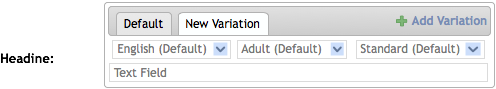
\includegraphics{variations-admin-interface-add-var.png}

Changing one of the dimensions changes the name of the tab.

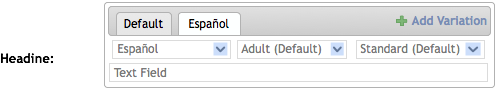
\includegraphics{variations-admin-interface-add-change1.png}

Changing another dimensions changes the name of the tab again.

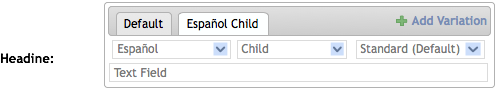
\includegraphics{variations-admin-interface-add-change2.png}


\subsection{Declaring Something Inappropriate}
\label{getting_started:declaring-something-inappropriate}
In some cases you may want to specifically exclude variants of a dimension from returning content. Content that is inappropriate for children is a good example.

To exclude content, simply create an empty variation. If you changed the Audience dimension to ``Child'' and left the field blank, then the template could properly display something like ``This content is inappropriate for children.''

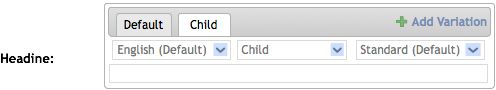
\includegraphics{variations-admin-interface-exclude.png}


\section{Configuring Models with Variations}
\label{getting_started:configuring-models-with-variations}

\subsection{Variations}
\label{getting_started:variations}

\section{Setting Up Search}
\label{getting_started:setting-up-search}

\chapter{Variations and URLs}
\label{variations_and_urls:variations-and-urls}\label{variations_and_urls::doc}
URLs are important. Content should exist at one and only one URL. Each variation in content needs to have a unique URL. Django Text Variation tries to be as flexible as possible by using middleware to check configured patterns as they are requested.


\section{Ways of Handling Variations in URLs}
\label{variations_and_urls:ways-of-handling-variations-in-urls}
A great resource for my research was
\href{http://h3h.net/technology/designing-urls-for-multilingual-websites}{this blog post} regarding methods for handling multilingual websites. He defines nine ways of accomplishing language variations in content, many of which are not generic enough for use here.

First and foremost, \href{http://googlewebmastercentral.blogspot.com/2010/03/working-with-multi-regional-websites.html}{query parameters are not recommended.} and will not be supported.

Ultimately, there are three ways specify a unique variation:
\begin{itemize}
\item {} 
Domain

\item {} 
Path segment

\item {} 
Path parameters or other delimited suffix

\end{itemize}

You can use any combination of these methods to specify your variation.


\subsection{Domain}
\label{variations_and_urls:domain}
The domain difference could be at the host level, such as \code{dim1.example.com} or at a different top-level domain such as \code{example.es}. Top-level domains are probably only useful for specifying language variations.

\begin{notice}{note}{Note:}
You can only vary on one dimension within a domain. That means you can vary on language (\code{en.example.com}) or audience (\code{kids.example.com}), but not both (\code{en.kids.example.com}) within the domain.
\end{notice}


\subsection{Path Segment}
\label{variations_and_urls:path-segment}
A common variation, especially for language specification, is to have the variant prefix the path, such as \code{www.example.com/en/} or \code{www.example.com/es/}. However, encoding the variant within the path (\code{www.example.com/blog/en/} ) is also supported.

\begin{notice}{note}{Note:}
Putting the variant within the path may make it difficult to re-create variation URLs of items. If the item's URL is either prefixed or suffixed with dimension information, the variation URL is easily created.
\end{notice}


\subsection{Path Parameters or Delimited Suffix}
\label{variations_and_urls:path-parameters-or-delimited-suffix}
Path parameters are defined by
\href{http://tools.ietf.org/html/rfc3986\#section-3.3}{Section 3.3 of RFC 3986}
as semicolon (;) and comma (,). One benefit of the semicolon is support within Python's urlparse module. It is also possible to use a dot (.) delimiter if you wish, although it is less common and not recommended.


\section{Defining the URL patterns}
\label{variations_and_urls:defining-the-url-patterns}

\subsection{Assigning a variant to a domain}
\label{variations_and_urls:assigning-a-variant-to-a-domain}
Domain variations are defined within each variant's dictionary. Each variant for each dimension has several options, one of which is domain. If domain is not specified, the default domain is assumed.


\subsection{Dimensions Within the Path}
\label{variations_and_urls:dimensions-within-the-path}
The middleware checks if the requested path fits a defined set of regular expressions in \code{TEXT\_VARIATIONS{[}'URL\_REGEXES'{]}}. To make the regular expressions easier to define, there are two shortcuts available.
\begin{description}
\item[{\textbf{\{\textless{}dimension\_name\textgreater{}\}}}] \leavevmode
This string will substitute a named group with every variant as an option. So \code{'\{language\}'} could result in \code{'(?P\textless{}language\textgreater{}en\textbar{}es\textbar{}es-mx\textbar{}fr)'}

\item[{\textbf{\{path\}}}] \leavevmode
This string will substitute a group to catch any character: \code{(.*)}

\end{description}


\subsection{Examples}
\label{variations_and_urls:examples}
Assuming two dimensions: `language' and `audience' with variants `en', `es', `es-mx', `fr' and `cd', `tn', `ad' respectively.

\begin{tabulary}{\linewidth}{|L|L|L|}
\hline
\textbf{
\#
} & \textbf{
RegEx Pattern
} & \textbf{
Result
}\\
\hline

1
 & 
\code{'\{language\}/\{path\};\{audience\}'}
 & 
\code{'(?P\textless{}language\textgreater{}en\textbar{}es\textbar{}es-mx\textbar{}fr)/(.*);(?P\textless{}audience\textgreater{}cd/tn/ad)'}
\\

2
 & 
\code{'\{path\}/\{language\}/\{path\};\{audience\}'}
 & 
\code{'(.*)/(?P\textless{}language\textgreater{}en\textbar{}es\textbar{}es-mx\textbar{}fr)/(.*);(?P\textless{}audience\textgreater{}cd/tn/ad)'}
\\

3
 & 
\code{'\{language\}/\{path\}\textbackslash{}.\{audience\}'}
 & 
\code{'(?P\textless{}language\textgreater{}en\textbar{}es\textbar{}es-mx\textbar{}fr)/(.*)\textbackslash{}.(?P\textless{}audience\textgreater{}cd/tn/ad)'}
\\
\hline
\end{tabulary}



\section{TextVariationMiddleware}
\label{variations_and_urls:textvariationmiddleware}
The middleware modifies the request
\begin{itemize}
\item {} 
Matches request path against the configured regular expressions

\item {} 
If it matches, extract the dimensions and set into \code{request.META{[}'TEXT\_VARIATIONS'{]}}

\item {} 
Join the unnamed groups in the matching regular expression with ``/''

\item {} 
Set \code{request.path}, \code{request.path\_info} and \code{request.META{[}'PATH\_INFO'{]}} to the resulting value

\end{itemize}

See {\hyperref[reference/middleware:textvariationmiddleware]{\emph{TextVariationMiddleware}}} for more detailed information.


\section{Requested Variation, Returned Variation and URLs}
\label{variations_and_urls:requested-variation-returned-variation-and-urls}\begin{itemize}
\item {} 
URLs without dimension information serve the default variation

\item {} 
URLS should either contain no variation information, or contain information for every dimension.

\item {} 
If a variant of one dimension is requested, the default variants of any other dimensions should be requested.

\item {} 
If a requested variation does not exist, a fallback variation is returned.

\item {} 
The Text Variation context processor will create a \code{text\_variations} variable with the variations returned for each field. If there are multiple variable fields in a model, you should pick one field to populate a \code{\textless{}link rel="canonical" href="" /\textgreater{}} tag.

\item {} 
The template could provide an alert on the page that the requested variation was not available and the substituted variation was.

\end{itemize}


\chapter{Templates}
\label{templates:templates}\label{templates::doc}
At the top of the page, you need to call a template tag to get the proper variation fit for the object

\begin{Verbatim}[commandchars=\\\{\}]
\PYG{c+cp}{\PYGZob{}\PYGZpc{}} \PYG{k}{get\PYGZus{}text\PYGZus{}variations} \PYG{n+nv}{object} \PYG{c+cp}{\PYGZpc{}\PYGZcb{}}
\end{Verbatim}

Default usage: get the best variation fit for the requested variation:

\begin{Verbatim}[commandchars=\\\{\}]
\PYG{c+cp}{\PYGZob{}\PYGZob{}} \PYG{n+nv}{object}\PYG{n+nv}{.headline\PYGZus{}variation} \PYG{c+cp}{\PYGZcb{}\PYGZcb{}}
\end{Verbatim}

Testing the requested variation/dimension

\begin{Verbatim}[commandchars=\\\{\}]
\PYG{c+cp}{\PYGZob{}\PYGZpc{}} \PYG{k}{if} \PYG{n+nv}{text\PYGZus{}variations}\PYG{n+nv}{.requested}\PYG{n+nv}{.language}\PYG{n+nv}{.code} \PYG{o}{==} \PYG{l+s+s1}{'es'} \PYG{c+cp}{\PYGZpc{}\PYGZcb{}}
\end{Verbatim}

Displaying information about the requested variation

\begin{Verbatim}[commandchars=\\\{\}]
\PYG{x}{\textless{}p\textgreater{}You are viewing the}
\PYG{c+cp}{\PYGZob{}\PYGZob{}} \PYG{n+nv}{text\PYGZus{}variations}\PYG{n+nv}{.requested}\PYG{n+nv}{.audience}\PYG{n+nv}{.name} \PYG{c+cp}{\PYGZcb{}\PYGZcb{}}
\PYG{x}{version of the site in}
\PYG{c+cp}{\PYGZob{}\PYGZob{}} \PYG{n+nv}{text\PYGZus{}variation}\PYG{n+nv}{.requested}\PYG{n+nv}{.language}\PYG{n+nv}{.name} \PYG{c+cp}{\PYGZcb{}\PYGZcb{}}\PYG{x}{.\textless{}/p\textgreater{}}
\end{Verbatim}

testing each field

\begin{Verbatim}[commandchars=\\\{\}]
\PYG{c+cp}{\PYGZob{}\PYGZpc{}} \PYG{k}{if} \PYG{n+nv}{text\PYGZus{}variations}\PYG{n+nv}{.headline}\PYG{n+nv}{.language}\PYG{n+nv}{.code} \PYG{o}{==} \PYG{l+s+s1}{'es'} \PYG{c+cp}{\PYGZpc{}\PYGZcb{}}
\end{Verbatim}

Testing if a field is not the requested variation

\begin{Verbatim}[commandchars=\\\{\}]
\PYG{c+cp}{\PYGZob{}\PYGZpc{}} \PYG{k}{if} \PYG{n+nv}{text\PYGZus{}variations}\PYG{n+nv}{.headline} \PYG{o}{==} \PYG{n+nv}{text\PYGZus{}variations}\PYG{n+nv}{.requested} \PYG{c+cp}{\PYGZpc{}\PYGZcb{}}
\end{Verbatim}

Does a specific variation exist for a field?

\begin{Verbatim}[commandchars=\\\{\}]
\PYG{c+cp}{\PYGZob{}\PYGZpc{}} \PYG{k}{if} \PYG{n+nv}{object}\PYG{n+nv}{.text\PYGZus{}variations}\PYG{n+nv}{.headline}\PYG{n+nv}{.en}\PYG{n+nv}{.ad} \PYG{c+cp}{\PYGZpc{}\PYGZcb{}}
\end{Verbatim}

get specific variation of a field

\begin{Verbatim}[commandchars=\\\{\}]
\PYG{c+cp}{\PYGZob{}\PYGZpc{}} \PYG{k}{get\PYGZus{}variation} \PYG{n+nv}{object} \PYG{n+nv}{headline} \PYG{n+nv}{language}\PYG{o}{=}\PYG{n+nv}{es} \PYG{c+cp}{\PYGZpc{}\PYGZcb{}}
\end{Verbatim}


\section{Context Processors}
\label{templates:context-processors}
\begin{Verbatim}[commandchars=\\\{\}]
\PYG{n}{text\PYGZus{}variations} \PYG{o}{=} \PYG{p}{\PYGZob{}}
    \PYG{l+s}{'}\PYG{l+s}{requested}\PYG{l+s}{'}\PYG{p}{:} \PYG{p}{\PYGZob{}}\PYG{l+s}{'}\PYG{l+s}{dim1}\PYG{l+s}{'}\PYG{p}{:} \PYG{p}{\PYGZob{}}\PYG{l+s}{'}\PYG{l+s}{code}\PYG{l+s}{'}\PYG{p}{:} \PYG{l+s}{'}\PYG{l+s}{c2}\PYG{l+s}{'}\PYG{p}{,} \PYG{l+s}{'}\PYG{l+s}{name}\PYG{l+s}{'}\PYG{p}{:} \PYG{l+s}{'}\PYG{l+s}{Code2}\PYG{l+s}{'}\PYG{p}{\PYGZcb{}}\PYG{p}{,}\PYG{p}{\PYGZcb{}}\PYG{p}{,}
    \PYG{l+s}{'}\PYG{l+s}{field1}\PYG{l+s}{'}\PYG{p}{:} \PYG{p}{\PYGZob{}}\PYG{l+s}{'}\PYG{l+s}{dim1}\PYG{l+s}{'}\PYG{p}{:} \PYG{p}{\PYGZob{}}\PYG{l+s}{'}\PYG{l+s}{code}\PYG{l+s}{'}\PYG{p}{:} \PYG{l+s}{'}\PYG{l+s}{co}\PYG{l+s}{'}\PYG{p}{,} \PYG{l+s}{'}\PYG{l+s}{name}\PYG{l+s}{'}\PYG{p}{:} \PYG{l+s}{'}\PYG{l+s}{Code1}\PYG{l+s}{'}\PYG{p}{\PYGZcb{}}\PYG{p}{,}\PYG{p}{\PYGZcb{}}\PYG{p}{,}
    \PYG{l+s}{'}\PYG{l+s}{field2}\PYG{l+s}{'}\PYG{p}{:} \PYG{p}{\PYGZob{}}\PYG{l+s}{'}\PYG{l+s}{dim1}\PYG{l+s}{'}\PYG{p}{:} \PYG{p}{\PYGZob{}}\PYG{l+s}{'}\PYG{l+s}{code}\PYG{l+s}{'}\PYG{p}{:} \PYG{l+s}{'}\PYG{l+s}{c2}\PYG{l+s}{'}\PYG{p}{,} \PYG{l+s}{'}\PYG{l+s}{name}\PYG{l+s}{'}\PYG{p}{:} \PYG{l+s}{'}\PYG{l+s}{Code2}\PYG{l+s}{'}\PYG{p}{\PYGZcb{}}\PYG{p}{,}\PYG{p}{\PYGZcb{}}
\PYG{p}{\PYGZcb{}}
\end{Verbatim}


\section{Canonical URLs}
\label{templates:canonical-urls}
When the returned variation does not match the requested variation

If there are multiple fields on a model with variations, each could have different set defined variations, you will have to pick one field to define the canonical variation, such as blog entry content.


\chapter{Editing One Dimension}
\label{editing_one_dimension::doc}\label{editing_one_dimension:editing-one-dimension}
In some cases the person who enters the content will not be the one who applies other variations. For example if the default language was English, there may be a person(s) who translate the content previously entered.

For these people, there is a different view on the content to make creating the variations easier.


\chapter{Reference}
\label{reference/index::doc}\label{reference/index:reference}

\section{Settings}
\label{reference/settings:id1}\label{reference/settings::doc}\label{reference/settings:settings}
All configuration for Django Text Variations occurs within the \code{TEXT\_VARIATIONS} setting variable. \code{TEXT\_VARIATIONS} is a dictionary with the following keys:
\begin{itemize}
\item {} 
{\hyperref[reference/settings:settings-dimensions]{\emph{DIMENSIONS}}}

\item {} 
{\hyperref[reference/settings:settings-dimension-priority]{\emph{DIMENSION\_PRIORITY}}}

\item {} 
{\hyperref[reference/settings:settings-models]{\emph{MODELS}}}

\item {} 
{\hyperref[reference/settings:settings-default-url-regex]{\emph{DEFAULT\_URL\_REGEX}}}

\item {} 
{\hyperref[reference/settings:settings-url-regex-map]{\emph{URL\_REGEX\_MAP}}}

\item {} 
{\hyperref[reference/settings:settings-example]{\emph{Example Settings}}}

\end{itemize}


\subsection{DIMENSIONS}
\label{reference/settings:settings-dimensions}\label{reference/settings:dimensions}

\subsection{DIMENSION\_PRIORITY}
\label{reference/settings:settings-dimension-priority}\label{reference/settings:dimension-priority}

\subsection{MODELS}
\label{reference/settings:models}\label{reference/settings:settings-models}

\subsection{DEFAULT\_URL\_REGEX}
\label{reference/settings:default-url-regex}\label{reference/settings:settings-default-url-regex}

\subsection{URL\_REGEX\_MAP}
\label{reference/settings:url-regex-map}\label{reference/settings:settings-url-regex-map}

\subsection{Example Settings}
\label{reference/settings:settings-example}\label{reference/settings:example-settings}
\begin{Verbatim}[commandchars=\\\{\}]
\PYG{n}{TEXT\PYGZus{}VARIATIONS} \PYG{o}{=} \PYG{p}{\PYGZob{}}
    \PYG{l+s}{'}\PYG{l+s}{DIMENSIONS}\PYG{l+s}{'}\PYG{p}{:} \PYG{p}{\PYGZob{}}
        \PYG{l+s}{'}\PYG{l+s}{audience}\PYG{l+s}{'}\PYG{p}{:} \PYG{p}{\PYGZob{}}
            \PYG{l+s}{'}\PYG{l+s}{ad}\PYG{l+s}{'}\PYG{p}{:} \PYG{p}{\PYGZob{}}
                \PYG{l+s}{'}\PYG{l+s}{name}\PYG{l+s}{'}\PYG{p}{:} \PYG{l+s}{u'}\PYG{l+s}{Adult}\PYG{l+s}{'}\PYG{p}{,}
                \PYG{l+s}{'}\PYG{l+s}{fallback}\PYG{l+s}{'}\PYG{p}{:} \PYG{n+nb+bp}{None}\PYG{p}{,}
            \PYG{p}{\PYGZcb{}}\PYG{p}{,}
            \PYG{l+s}{'}\PYG{l+s}{tn}\PYG{l+s}{'}\PYG{p}{:} \PYG{p}{\PYGZob{}}
                \PYG{l+s}{'}\PYG{l+s}{name}\PYG{l+s}{'}\PYG{p}{:} \PYG{l+s}{u'}\PYG{l+s}{Teen}\PYG{l+s}{'}\PYG{p}{,}
                \PYG{l+s}{'}\PYG{l+s}{fallback}\PYG{l+s}{'}\PYG{p}{:} \PYG{l+s}{'}\PYG{l+s}{ad}\PYG{l+s}{'}\PYG{p}{,}
            \PYG{p}{\PYGZcb{}}\PYG{p}{,}
            \PYG{l+s}{'}\PYG{l+s}{cd}\PYG{l+s}{'}\PYG{p}{:} \PYG{p}{\PYGZob{}}
                \PYG{l+s}{'}\PYG{l+s}{name}\PYG{l+s}{'}\PYG{p}{:} \PYG{l+s}{u'}\PYG{l+s}{Child}\PYG{l+s}{'}\PYG{p}{,}
                \PYG{l+s}{'}\PYG{l+s}{fallback}\PYG{l+s}{'}\PYG{p}{:} \PYG{l+s}{'}\PYG{l+s}{tn}\PYG{l+s}{'}\PYG{p}{,}
            \PYG{p}{\PYGZcb{}}
        \PYG{p}{\PYGZcb{}}\PYG{p}{,}
        \PYG{l+s}{'}\PYG{l+s}{text\PYGZus{}dificulty}\PYG{l+s}{'}\PYG{p}{:} \PYG{p}{\PYGZob{}}
            \PYG{l+s}{'}\PYG{l+s}{l}\PYG{l+s}{'}\PYG{p}{:} \PYG{p}{\PYGZob{}}
                \PYG{l+s}{'}\PYG{l+s}{name}\PYG{l+s}{'}\PYG{p}{:} \PYG{l+s}{u'}\PYG{l+s}{Low}\PYG{l+s}{'}\PYG{p}{,}
                \PYG{l+s}{'}\PYG{l+s}{fallback}\PYG{l+s}{'}\PYG{p}{:} \PYG{l+s}{'}\PYG{l+s}{s}\PYG{l+s}{'}\PYG{p}{,}
            \PYG{p}{\PYGZcb{}}\PYG{p}{,}
            \PYG{l+s}{'}\PYG{l+s}{s}\PYG{l+s}{'}\PYG{p}{:} \PYG{p}{\PYGZob{}}
                \PYG{l+s}{'}\PYG{l+s}{name}\PYG{l+s}{'}\PYG{p}{:} \PYG{l+s}{u'}\PYG{l+s}{Standard}\PYG{l+s}{'}\PYG{p}{,}
                \PYG{l+s}{'}\PYG{l+s}{fallback}\PYG{l+s}{'}\PYG{p}{:} \PYG{n+nb+bp}{None}\PYG{p}{,}
            \PYG{p}{\PYGZcb{}}\PYG{p}{,}
            \PYG{l+s}{'}\PYG{l+s}{a}\PYG{l+s}{'}\PYG{p}{:} \PYG{p}{\PYGZob{}}
                \PYG{l+s}{'}\PYG{l+s}{name}\PYG{l+s}{'}\PYG{p}{:} \PYG{l+s}{u'}\PYG{l+s}{Advanced}\PYG{l+s}{'}\PYG{p}{,}
                \PYG{l+s}{'}\PYG{l+s}{fallback}\PYG{l+s}{'}\PYG{p}{:} \PYG{l+s}{'}\PYG{l+s}{s}\PYG{l+s}{'}\PYG{p}{,}
            \PYG{p}{\PYGZcb{}}
        \PYG{p}{\PYGZcb{}}\PYG{p}{,}
        \PYG{l+s}{'}\PYG{l+s}{language}\PYG{l+s}{'}\PYG{p}{:} \PYG{p}{\PYGZob{}}
            \PYG{l+s}{'}\PYG{l+s}{en}\PYG{l+s}{'}\PYG{p}{:} \PYG{p}{\PYGZob{}}
                \PYG{l+s}{'}\PYG{l+s}{name}\PYG{l+s}{'}\PYG{p}{:} \PYG{l+s}{u'}\PYG{l+s}{English}\PYG{l+s}{'}\PYG{p}{,}
                \PYG{l+s}{'}\PYG{l+s}{fallback}\PYG{l+s}{'}\PYG{p}{:} \PYG{n+nb+bp}{None}\PYG{p}{,}
            \PYG{p}{\PYGZcb{}}\PYG{p}{,}
            \PYG{l+s}{'}\PYG{l+s}{es}\PYG{l+s}{'}\PYG{p}{:} \PYG{p}{\PYGZob{}}
                \PYG{l+s}{'}\PYG{l+s}{name}\PYG{l+s}{'}\PYG{p}{:} \PYG{l+s}{u'}\PYG{l+s}{Español}\PYG{l+s}{'}\PYG{p}{,}
                \PYG{l+s}{'}\PYG{l+s}{fallback}\PYG{l+s}{'}\PYG{p}{:} \PYG{l+s}{'}\PYG{l+s}{en}\PYG{l+s}{'}\PYG{p}{,}
                \PYG{l+s}{'}\PYG{l+s}{domain}\PYG{l+s}{'}\PYG{p}{:} \PYG{l+s}{'}\PYG{l+s}{es.example.com}\PYG{l+s}{'}\PYG{p}{,}
            \PYG{p}{\PYGZcb{}}\PYG{p}{,}
            \PYG{l+s}{'}\PYG{l+s}{es-mx}\PYG{l+s}{'}\PYG{p}{:} \PYG{p}{\PYGZob{}}
                \PYG{l+s}{'}\PYG{l+s}{name}\PYG{l+s}{'}\PYG{p}{:} \PYG{l+s}{u'}\PYG{l+s}{Español mexicano}\PYG{l+s}{'}\PYG{p}{,}
                \PYG{l+s}{'}\PYG{l+s}{fallback}\PYG{l+s}{'}\PYG{p}{:} \PYG{l+s}{'}\PYG{l+s}{es}\PYG{l+s}{'}\PYG{p}{,}
                \PYG{l+s}{'}\PYG{l+s}{domain}\PYG{l+s}{'}\PYG{p}{:} \PYG{l+s}{'}\PYG{l+s}{es-mx.example.com}\PYG{l+s}{'}\PYG{p}{,}
            \PYG{p}{\PYGZcb{}}\PYG{p}{,}
            \PYG{l+s}{'}\PYG{l+s}{fr}\PYG{l+s}{'}\PYG{p}{:} \PYG{p}{\PYGZob{}}
                \PYG{l+s}{'}\PYG{l+s}{name}\PYG{l+s}{'}\PYG{p}{:} \PYG{l+s}{u'}\PYG{l+s}{Français}\PYG{l+s}{'}\PYG{p}{,}
                \PYG{l+s}{'}\PYG{l+s}{fallback}\PYG{l+s}{'}\PYG{p}{:} \PYG{l+s}{'}\PYG{l+s}{en}\PYG{l+s}{'}\PYG{p}{,}
                \PYG{l+s}{'}\PYG{l+s}{domain}\PYG{l+s}{'}\PYG{p}{:} \PYG{l+s}{'}\PYG{l+s}{fr.example.com}\PYG{l+s}{'}\PYG{p}{,}
            \PYG{p}{\PYGZcb{}}
        \PYG{p}{\PYGZcb{}}\PYG{p}{,}
    \PYG{p}{\PYGZcb{}}\PYG{p}{,}
    \PYG{l+s}{'}\PYG{l+s}{DIMENSION\PYGZus{}PRIORITY}\PYG{l+s}{'}\PYG{p}{:} \PYG{p}{[}\PYG{l+s}{'}\PYG{l+s}{language}\PYG{l+s}{'}\PYG{p}{,} \PYG{l+s}{'}\PYG{l+s}{audience}\PYG{l+s}{'}\PYG{p}{,} \PYG{l+s}{'}\PYG{l+s}{text\PYGZus{}difficulty}\PYG{l+s}{'}\PYG{p}{]}\PYG{p}{,}
    \PYG{l+s}{'}\PYG{l+s}{MODELS}\PYG{l+s}{'}\PYG{p}{:} \PYG{p}{\PYGZob{}}
        \PYG{l+s}{'}\PYG{l+s}{app.model}\PYG{l+s}{'}\PYG{p}{:} \PYG{p}{[}\PYG{l+s}{'}\PYG{l+s}{field1}\PYG{l+s}{'}\PYG{p}{,} \PYG{l+s}{'}\PYG{l+s}{field2}\PYG{l+s}{'}\PYG{p}{]}\PYG{p}{,}
        \PYG{l+s}{'}\PYG{l+s}{app2.model}\PYG{l+s}{'}\PYG{p}{:} \PYG{p}{[}\PYG{l+s}{'}\PYG{l+s}{field1}\PYG{l+s}{'}\PYG{p}{,} \PYG{p}{]}
    \PYG{p}{\PYGZcb{}}\PYG{p}{,}
    \PYG{l+s}{'}\PYG{l+s}{DEFAULT\PYGZus{}URL\PYGZus{}REGEX}\PYG{l+s}{'}\PYG{p}{:} \PYG{l+s}{'}\PYG{l+s}{\PYGZob{}language\PYGZcb{}/\PYGZob{}path\PYGZcb{};\PYGZob{}audience\PYGZcb{},\PYGZob{}text\PYGZus{}difficulty\PYGZcb{}}\PYG{l+s}{'}\PYG{p}{,}
    \PYG{l+s}{'}\PYG{l+s}{URL\PYGZus{}REGEX\PYGZus{}MAP}\PYG{l+s}{'}\PYG{p}{:} \PYG{p}{\PYGZob{}}
        \PYG{l+s}{'}\PYG{l+s}{app.model}\PYG{l+s}{'}\PYG{p}{:} \PYG{l+s}{'}\PYG{l+s}{\PYGZob{}path\PYGZcb{};\PYGZob{}language\PYGZcb{},\PYGZob{}audience\PYGZcb{},\PYGZob{}text\PYGZus{}difficulty\PYGZcb{}}\PYG{l+s}{'}\PYG{p}{,}
    \PYG{p}{\PYGZcb{}}
\PYG{p}{\PYGZcb{}}
\end{Verbatim}


\section{Implementation Notes}
\label{reference/implementation_notes:implementation-notes}\label{reference/implementation_notes::doc}\begin{enumerate}
\item {} 
There could be potentially a large number of variations for an individual field.

\item {} 
We want to keep the number of database calls/accesses and data storage to a minimum.

\item {} 
We must track some metadata about the variations, such as: variations used, invalidated variations.

\end{enumerate}


\subsection{Methods}
\label{reference/implementation_notes:methods}\begin{enumerate}
\item {} \begin{description}
\item[{Related table(s)}] \leavevmode
There are several variations:
\begin{itemize}
\item {} 
One table for each model with variations (using a Foreign Key)

\item {} 
One table for all models with variations (using a Generic Foreign Key)

\item {} 
Use a JSON field for all text variations of an object

\item {} 
A separate row for each text variation

\end{itemize}

\end{description}

\item {} \begin{description}
\item[{Additional field(s) in the model}] \leavevmode
There are two variations:
\begin{itemize}
\item {} 
Use a JSON field for all text variations of an object

\item {} 
A separate field for each potential text variation

\end{itemize}

\end{description}

\end{enumerate}


\subsection{Implementation}
\label{reference/implementation_notes:implementation}
A combination of both methods will be used in a non-normalized way to provide flexibility and performance. A variation table for each model with variations will store each variation for each field. A JSON/serialized field on the model will store a cached version of the same information.

The fields in the variation table are:

\begin{tabulary}{\linewidth}{|L|L|}
\hline
\textbf{
field
} & \textbf{
Description
}\\
\hline

\textless{}model\textgreater{}\_id
 & 
Foreign key to the row in the master table
\\

fieldname
 & 
Name of the field in which this variation applies
\\

\textless{}name\textgreater{}\_dim
 & 
A field for each defined dimension to contain the dimension variant
\\

is\_invalid
 & 
A boolean flag to indicate the variation is currently invalid, as the default variation has changed. Declaring variations invalid instead of deleting them should be an option as to allow the site to continue to display the content.
\\

value
 & 
The value of this variation for this field
\\
\hline
\end{tabulary}


The cache field contains a structure based on the current {\hyperref[reference/settings:settings-dimension-priority]{\emph{DIMENSION\_PRIORITY}}} settings.

\begin{notice}{warning}{Warning:}
If this setting changes the cache field for each item in every table will need to be recalculated. There is a management command to do this.
\end{notice}

The cache is a hierarchical dictionary with each field at the top level and then each dimension hierarchically contained in order of priority.

\begin{Verbatim}[commandchars=\\\{\}]
\PYG{p}{\PYGZob{}}
    \PYG{l+s}{'}\PYG{l+s}{field}\PYG{l+s}{'}\PYG{p}{:} \PYG{p}{\PYGZob{}}
        \PYG{l+s}{'}\PYG{l+s}{dim1-variant1}\PYG{l+s}{'}\PYG{p}{:} \PYG{p}{\PYGZob{}}
            \PYG{l+s}{'}\PYG{l+s}{dim2-variant1}\PYG{l+s}{'}\PYG{p}{:} \PYG{l+s}{'}\PYG{l+s}{variation value}\PYG{l+s}{'}\PYG{p}{,}
            \PYG{l+s}{'}\PYG{l+s}{dim2-variant2}\PYG{l+s}{'}\PYG{p}{:} \PYG{l+s}{'}\PYG{l+s}{variation value}\PYG{l+s}{'}\PYG{p}{,}
        \PYG{p}{\PYGZcb{}}
    \PYG{p}{\PYGZcb{}}
\PYG{p}{\PYGZcb{}}
\end{Verbatim}


\subsection{Example Walkthrough}
\label{reference/implementation_notes:example-walkthrough}
Assuming that we have three dimensions: audience, text difficulty, and language; a table called article with three variable fields: headline, subhead, and content; the table and metadata table might look like:

\begin{notice}{note}{Note:}
See {\hyperref[reference/settings:settings-example]{\emph{Example Settings}}} for the configuration.
\end{notice}

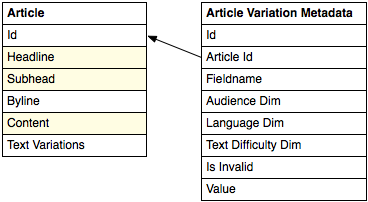
\includegraphics{variations-schema-example.png}

If you added a row into article, you might have

\begin{tabulary}{\linewidth}{|L|L|L|L|L|L|}
\hline
\textbf{
Id
} & \textbf{
Headline
} & \textbf{
Subhead
} & \textbf{
Byline
} & \textbf{
Content
} & \textbf{
Text Variations
}\\
\hline

1
 & 
First article
 &  & 
Carmen
 & 
Lots of ...
 & 
\code{\{'headline':\{'en':\{'ad'...}
\\
\hline
\end{tabulary}


The Text Variations field would contain a serialized dictionary:

\begin{Verbatim}[commandchars=\\\{\}]
\PYG{p}{\PYGZob{}}
    \PYG{l+s}{'}\PYG{l+s}{headline}\PYG{l+s}{'}\PYG{p}{:} \PYG{p}{\PYGZob{}}
        \PYG{l+s}{'}\PYG{l+s}{en}\PYG{l+s}{'}\PYG{p}{:} \PYG{p}{\PYGZob{}} \PYG{l+s}{'}\PYG{l+s}{ad}\PYG{l+s}{'}\PYG{p}{:} \PYG{p}{\PYGZob{}} \PYG{l+s}{'}\PYG{l+s}{s}\PYG{l+s}{'}\PYG{p}{:} \PYG{l+s}{'}\PYG{l+s}{First Article}\PYG{l+s}{'}\PYG{p}{,}\PYG{p}{\PYGZcb{}}\PYG{p}{,}\PYG{p}{\PYGZcb{}}\PYG{p}{,}\PYG{p}{\PYGZcb{}}\PYG{p}{,}
    \PYG{l+s}{'}\PYG{l+s}{subhead}\PYG{l+s}{'}\PYG{p}{:} \PYG{p}{\PYGZob{}}
        \PYG{l+s}{'}\PYG{l+s}{en}\PYG{l+s}{'}\PYG{p}{:} \PYG{p}{\PYGZob{}} \PYG{l+s}{'}\PYG{l+s}{ad}\PYG{l+s}{'}\PYG{p}{:} \PYG{p}{\PYGZob{}} \PYG{l+s}{'}\PYG{l+s}{s}\PYG{l+s}{'}\PYG{p}{:} \PYG{l+s}{'}\PYG{l+s}{'}\PYG{p}{,}\PYG{p}{\PYGZcb{}}\PYG{p}{,}\PYG{p}{\PYGZcb{}}\PYG{p}{,}\PYG{p}{\PYGZcb{}}\PYG{p}{,}
    \PYG{l+s}{'}\PYG{l+s}{content}\PYG{l+s}{'}\PYG{p}{:} \PYG{p}{\PYGZob{}}
        \PYG{l+s}{'}\PYG{l+s}{en}\PYG{l+s}{'}\PYG{p}{:} \PYG{p}{\PYGZob{}} \PYG{l+s}{'}\PYG{l+s}{ad}\PYG{l+s}{'}\PYG{p}{:} \PYG{p}{\PYGZob{}} \PYG{l+s}{'}\PYG{l+s}{s}\PYG{l+s}{'}\PYG{p}{:} \PYG{l+s}{'}\PYG{l+s}{Lots of ...}\PYG{l+s}{'}\PYG{p}{,}\PYG{p}{\PYGZcb{}}\PYG{p}{,}\PYG{p}{\PYGZcb{}}\PYG{p}{,}\PYG{p}{\PYGZcb{}}\PYG{p}{,}
\PYG{p}{\PYGZcb{}}
\end{Verbatim}

And the Audience Variation table contains

\begin{tabulary}{\linewidth}{|L|L|L|L|L|L|L|L|}
\hline
\textbf{
Id
} & \textbf{
Article Id
} & \textbf{
Fieldname
} & \textbf{
Audience Dim
} & \textbf{
Language Dim
} & \textbf{
Text Difficulty Dim
} & \textbf{
Is Invalid
} & \textbf{
Value
}\\
\hline

1
 & 
1
 & 
headline
 & 
ad
 & 
en
 & 
s
 & 
False
 & 
First Article
\\

2
 & 
1
 & 
subhead
 & 
ad
 & 
en
 & 
s
 & 
False
 & \\

3
 & 
1
 & 
content
 & 
ad
 & 
en
 & 
s
 & 
False
 & 
Lots of ...
\\
\hline
\end{tabulary}


If you add a spanish variation to the headline and content fields, the Text Variations field would contain:

\begin{Verbatim}[commandchars=\\\{\}]
\PYG{p}{\PYGZob{}}
    \PYG{l+s}{'}\PYG{l+s}{headline}\PYG{l+s}{'}\PYG{p}{:} \PYG{p}{\PYGZob{}}
        \PYG{l+s}{'}\PYG{l+s}{en}\PYG{l+s}{'}\PYG{p}{:} \PYG{p}{\PYGZob{}} \PYG{l+s}{'}\PYG{l+s}{ad}\PYG{l+s}{'}\PYG{p}{:} \PYG{p}{\PYGZob{}} \PYG{l+s}{'}\PYG{l+s}{s}\PYG{l+s}{'}\PYG{p}{:} \PYG{l+s}{'}\PYG{l+s}{First Article}\PYG{l+s}{'}\PYG{p}{,}\PYG{p}{\PYGZcb{}}\PYG{p}{,}\PYG{p}{\PYGZcb{}}\PYG{p}{,}
        \PYG{l+s}{'}\PYG{l+s}{es}\PYG{l+s}{'}\PYG{p}{:} \PYG{p}{\PYGZob{}} \PYG{l+s}{'}\PYG{l+s}{ad}\PYG{l+s}{'}\PYG{p}{:} \PYG{p}{\PYGZob{}} \PYG{l+s}{'}\PYG{l+s}{s}\PYG{l+s}{'}\PYG{p}{:} \PYG{l+s}{u'}\PYG{l+s}{Artículo Primero}\PYG{l+s}{'}\PYG{p}{,}\PYG{p}{\PYGZcb{}}\PYG{p}{,}\PYG{p}{\PYGZcb{}}\PYG{p}{,}\PYG{p}{\PYGZcb{}}\PYG{p}{,}
    \PYG{l+s}{'}\PYG{l+s}{subhead}\PYG{l+s}{'}\PYG{p}{:} \PYG{p}{\PYGZob{}}
        \PYG{l+s}{'}\PYG{l+s}{en}\PYG{l+s}{'}\PYG{p}{:} \PYG{p}{\PYGZob{}} \PYG{l+s}{'}\PYG{l+s}{ad}\PYG{l+s}{'}\PYG{p}{:} \PYG{p}{\PYGZob{}} \PYG{l+s}{'}\PYG{l+s}{s}\PYG{l+s}{'}\PYG{p}{:} \PYG{l+s}{'}\PYG{l+s}{'}\PYG{p}{,}\PYG{p}{\PYGZcb{}}\PYG{p}{,}\PYG{p}{\PYGZcb{}}\PYG{p}{,}\PYG{p}{\PYGZcb{}}\PYG{p}{,}
    \PYG{l+s}{'}\PYG{l+s}{content}\PYG{l+s}{'}\PYG{p}{:} \PYG{p}{\PYGZob{}}
        \PYG{l+s}{'}\PYG{l+s}{en}\PYG{l+s}{'}\PYG{p}{:} \PYG{p}{\PYGZob{}} \PYG{l+s}{'}\PYG{l+s}{ad}\PYG{l+s}{'}\PYG{p}{:} \PYG{p}{\PYGZob{}} \PYG{l+s}{'}\PYG{l+s}{s}\PYG{l+s}{'}\PYG{p}{:} \PYG{l+s}{'}\PYG{l+s}{Lots of ...}\PYG{l+s}{'}\PYG{p}{,}\PYG{p}{\PYGZcb{}}\PYG{p}{,}\PYG{p}{\PYGZcb{}}\PYG{p}{,}
        \PYG{l+s}{'}\PYG{l+s}{es}\PYG{l+s}{'}\PYG{p}{:} \PYG{p}{\PYGZob{}} \PYG{l+s}{'}\PYG{l+s}{ad}\PYG{l+s}{'}\PYG{p}{:} \PYG{p}{\PYGZob{}} \PYG{l+s}{'}\PYG{l+s}{s}\PYG{l+s}{'}\PYG{p}{:} \PYG{l+s}{'}\PYG{l+s}{Mucho ...}\PYG{l+s}{'}\PYG{p}{,}\PYG{p}{\PYGZcb{}}\PYG{p}{,}\PYG{p}{\PYGZcb{}}\PYG{p}{,}\PYG{p}{\PYGZcb{}}\PYG{p}{,}
\PYG{p}{\PYGZcb{}}
\end{Verbatim}

And the Audience Variation table contains

\begin{tabulary}{\linewidth}{|L|L|L|L|L|L|L|L|}
\hline
\textbf{
Id
} & \textbf{
Article Id
} & \textbf{
Fieldname
} & \textbf{
Audience Dim
} & \textbf{
Language Dim
} & \textbf{
Text Difficulty Dim
} & \textbf{
Is Invalid
} & \textbf{
Value
}\\
\hline

1
 & 
1
 & 
headline
 & 
ad
 & 
en
 & 
s
 & 
False
 & 
First Article
\\

2
 & 
1
 & 
subhead
 & 
ad
 & 
en
 & 
s
 & 
False
 & \\

3
 & 
1
 & 
content
 & 
ad
 & 
en
 & 
s
 & 
False
 & 
Lots of ...
\\

4
 & 
1
 & 
headline
 & 
ad
 & 
es
 & 
s
 & 
False
 & 
Artículo Primero
\\

5
 & 
1
 & 
content
 & 
ad
 & 
es
 & 
s
 & 
False
 & 
Mucho ...
\\
\hline
\end{tabulary}



\subsection{Schema Migrations}
\label{reference/implementation_notes:schema-migrations}
Adding/removing the JSON field

Adding/removing a metadata dimension field


\section{Management Commands}
\label{reference/management_commands:management-commands}\label{reference/management_commands::doc}

\section{Template Tags}
\label{reference/template_tags::doc}\label{reference/template_tags:template-tags}
\{\% variation\_url object variation \%\}

returns a url of the object with variations applied to it

\{\% get\_text\_variations object \%\}

Using the request, or other method, if possible, set the object's \textless{}field\textgreater{}\_variation attributes and possibly update the text\_variations context variable

Required before using the content object.

\{\% get\_variation object field dimension=val dimension2=val ... \%\}

Returns the best variation fit for the object's specified field


\section{TextVariationMiddleware}
\label{reference/middleware:textvariationmiddleware}\label{reference/middleware::doc}\label{reference/middleware:id1}
Needs to be first in the list so it can properly modify the path information.

The middleware modifies the request
\begin{itemize}
\item {} 
Matches request path against the configured regular expressions

\item {} 
If it matches, extract the dimensions and set into request.META{[}'TEXT\_VARIATIONS'{]}

\item {} 
Join the unnamed groups in the matching regular expression with ``/''

\item {} 
Set request.path, request.path\_info and request.META{[}'PATH\_INFO'{]} to the resulting value

\end{itemize}


\section{Object Methods}
\label{reference/object_methods::doc}\label{reference/object_methods:object-methods}
get\_FIELD\_variation (dimension=val, dimension2=val, ...)

pulls the variation for FIELD that fits the requested dimension values. Dimensions not specified are assumed to be the default. Will fall back to default variation if none exist.


\chapter{Items for Future Versions}
\label{future_versions::doc}\label{future_versions:items-for-future-versions}\begin{itemize}
\item {} 
Configurable storage engine for variation storage, to allow for example:
\begin{itemize}
\item {} 
hstore in PostgreSQL

\item {} 
segmentation of variations (e.g. a field for each language which stores variations)

\end{itemize}

\end{itemize}


\chapter{Indices and tables}
\label{index:indices-and-tables}\begin{itemize}
\item {} 
\emph{genindex}

\item {} 
\emph{modindex}

\item {} 
\emph{search}

\end{itemize}



\renewcommand{\indexname}{Index}
\printindex
\end{document}
